 \chapter{Trigonometria}

 \section{Triângulo retângulo}

  Considere o triângulo retângulo, (triângulo que possui um de seus ângulos internos medindo $90 \degree$), como na figura abaixo:
  \begin{figure}[H]
   \centering
   \fbox{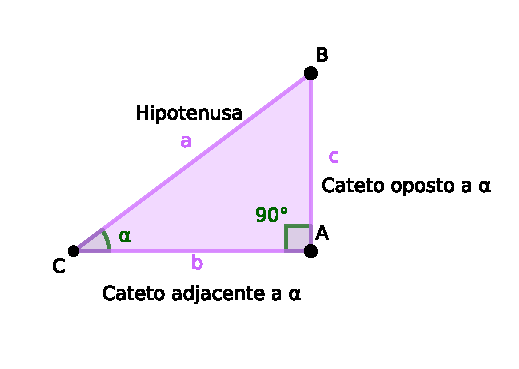
\includegraphics[width=7cm]{Capitulos/Figuras/triangulo_retangulo.pdf}}
   \caption{Triângulo retângulo}
  \end{figure}
 para este triângulo temos que é válido o seguinte teorema:

 \vskip0.3cm

\colorbox{azul}{
 \begin{minipage}{0.9\linewidth}
 \begin{center}
 \textbf{Teorema de Pitágoras}
  \[a^2= b^2 + c^2.\]
 \end{center}
 \end{minipage}}

 \vskip0.3cm

 Este é um resultado importante, já que com ele é possível encontrar o valor de um dos lados do triângulo, nos casos em que não temos todos os lados dados.

 Para este triângulo, as funções seno, cosseno e tangente são dadas pelas seguintes razões trigonométricas, nesta ordem:

 \vskip0.3cm

\colorbox{azul}{
 \begin{minipage}{0.9\linewidth}
 \begin{center}
 \textbf{Funções trigonométricas}
  \begin{eqnarray*}
   \sen(\alpha)= \frac{c}{a}= \frac{CO}{HI} \ ; \ \
   \cos(\alpha)= \frac{b}{a}= \frac{CA}{HI} \ ; \ \
   \tan(\alpha)= \frac{c}{b}= \frac{CO}{CA}.
 \end{eqnarray*}
 \end{center}
 \end{minipage}}

 \vskip0.3cm

 Como a soma dos ângulos internos de um triângulo é $180 \degree$, e estamos aqui tratando de um triângulo retângulo, decorre que neste caso $0 \degree \leqslant \alpha \leqslant 90 \degree$. Porém estas funções estão definidas para qualquer número real, mas para um primeiro estudo é suficiente conhecer seus valores para os ângulos $0 \degree \leqslant \alpha \leqslant 360 \degree$.

 Destacamos aqui os valores do seno, cosseno e tangente dos \emph{ângulos notáveis} que são os mais utilizados:

 \begin{table}[H]
 \centering
 \begin{tabular}{|c|c|c|c|c|c|} \hline
 \rowcolor{cinza}
               & $0 \degree$  & $30 \degree$  & $45 \degree$  & $60 \degree$ & $90 \degree$  \\\hline
  $\pmb{\sen}$ & $0$ &$\frac{1}{2}$ & $\frac{\sqrt{2}}{2}$ & $\frac{\sqrt{3}}{2}$ & $1$ \\\hline
  $\pmb{\cos}$ & $1$ & $\frac{\sqrt{3}}{2}$ & $\frac{\sqrt{2}}{2}$ & $\frac{1}{2}$ & $0$ \\\hline
  $\pmb{\tan}$ & $0$ & $\frac{\sqrt{3}}{3}$ & $1$ & $\sqrt{3}$ & $\nexists$ \\\hline
 \end{tabular}
\end{table}
 Na próxima seção veremos como utilizar estes valores para calcular seno, cosseno e tangente de ângulos maiores que $90 \degree$.

\section{Círculo trigonométrico}

 No plano cartesiano, consideremos um círculo de centro na origem e raio $1$, neste círculo representamos as imagens das funções trigonométricas aplicadas à  $0 \degree \leqslant \alpha \leqslant 360 \degree$. Como mostra a seguinte figura:
 \begin{figure}[H]
   \centering
   \fbox{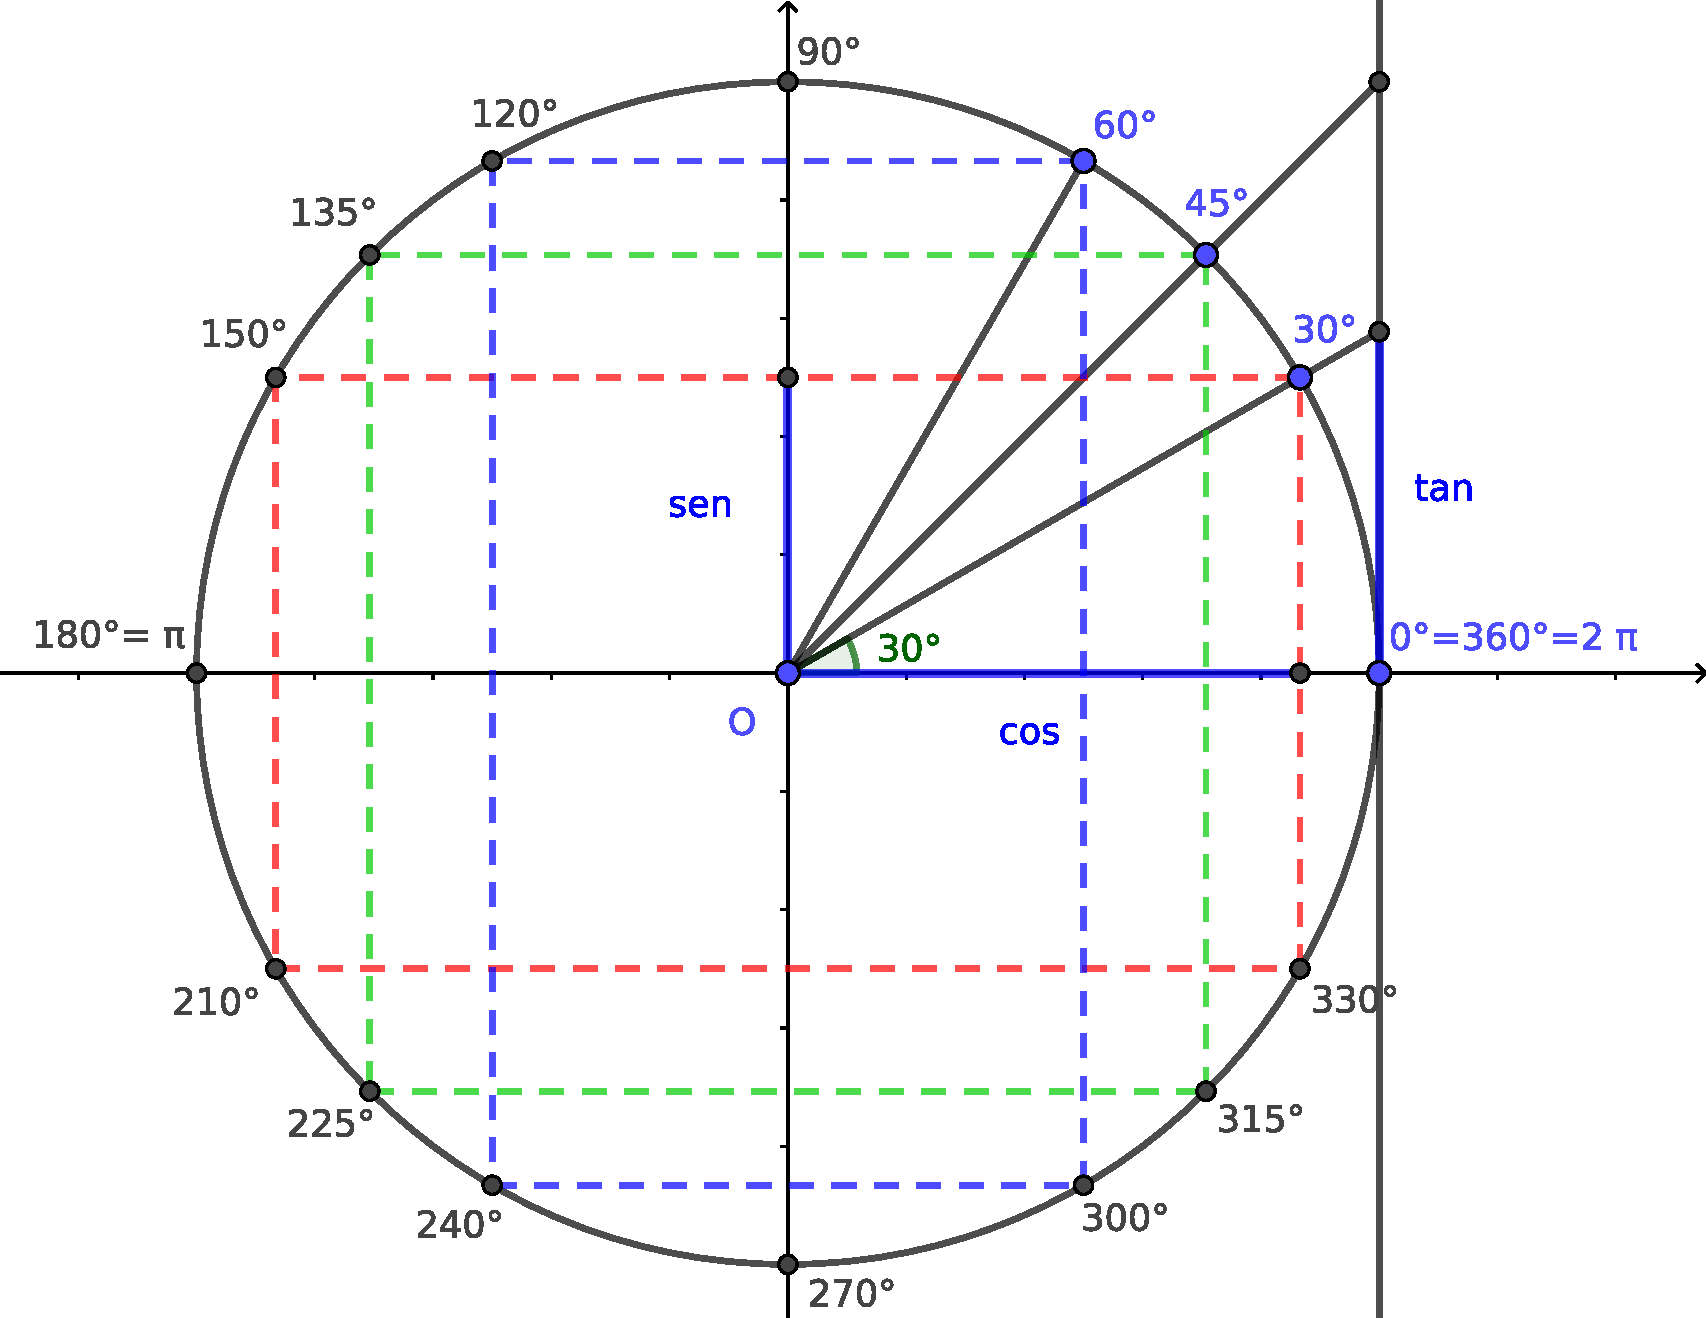
\includegraphics[width=9cm]{Capitulos/Figuras/circulo_trigonometrico.pdf}}
   \caption{Círculo trigonométrico}
  \end{figure}

  A partir do círculo trigonométrico concluímos que:

  \begin{table}[H]
 \centering
 \begin{tabular}{|c|c|c|c|} \hline
 \rowcolor{cinza}
               &  $120\degree$  & $135\degree$  &  $150\degree$ \\\hline
  $\pmb{\sen}$ & $\sen(60\degree)$ &$\sen(45\degree)$ & $\sen(30\degree)$  \\\hline
  $\pmb{\cos}$ & $-\cos(60\degree)$ &$-\cos(45\degree)$ & $-\cos(30\degree)$  \\\hline
  $\pmb{\tan}$ & $-\tan(60\degree)$ &$-\tan(45\degree)$ & $-\tan(30\degree)$  \\\hline
 \end{tabular}
\end{table}

 \begin{table}[H]
 \centering
 \begin{tabular}{|c|c|c|c|} \hline
 \rowcolor{cinza}
                & $210\degree$ & $225\degree$  & $240\degree$  \\\hline
  $\pmb{\sen}$ &  $-\sen(30\degree)$ & $-\sen(45\degree)$ & $-\sen(60\degree)$  \\\hline
  $\pmb{\cos}$ &  $-\cos(30\degree)$ & $-\cos(45\degree)$ & $-\cos(60\degree)$  \\\hline
  $\pmb{\tan}$ &  $\tan(30\degree)$ & $\tan(45\degree)$ & $\tan(60\degree)$   \\\hline
 \end{tabular}
\end{table}

 \begin{table}[h]
 \centering
 \begin{tabular}{|c|c|c|c|} \hline
 \rowcolor{cinza}
               & $300\degree$ & $315\degree$ & $330\degree$ \\\hline
  $\pmb{\sen}$ & $\sen(60\degree)$ & $\sen(45\degree)$ & $\sen(30\degree)$ \\\hline
  $\pmb{\cos}$ & $\cos(60\degree)$ & $\cos(45\degree)$ & $\cos(30\degree)$  \\\hline
  $\pmb{\tan}$ & $-\tan(60\degree)$ & $-\tan(45\degree)$ & $-\tan(30\degree)$  \\\hline
 \end{tabular}
\end{table}


  Os ângulos podem também ser representados em radianos, respeitando a seguinte relação:

  \[\destaque{\pi \text{ radianos}= 180 \degree}\]

  Usando esta relação podemos transformar graus para radianos e radianos para graus, vamos ver dois exemplos:

  \begin{exem}
   Qual a medida em graus do ângulo que mede $\frac{\pi}{4} rad$?

   \underline{Resolução:}

   Sabemos que $\pi rad= 180\degree$, portanto usando a regra de 3 abaixo conseguimos encontrar o valor em graus deste ângulo:
   \begin{eqnarray*}
  \text{Graus} & & \text{Radianos} \\
   180 & = & \pi\\
  x & = & \frac{\pi}{4}
 \end{eqnarray*}
 usando a propriedade da proporcionalidade, ou seja, multiplicando cruzado temos:

 $180 \cdot \frac{\pi}{4}= \pi \cdot x \Rightarrow \pi \cdot x= \frac{180 \pi}{4} \Rightarrow x= \frac{45 \pi}{\pi} \Rightarrow x= 45\degree$.

 \fim
  \end{exem}

  \begin{exem}
   Qual a medida em radianos do ângulo que mede $30\degree$?

   \underline{Resolução:}

   Sabemos que $\pi rad= 180\degree$, portanto usando a regra de 3 abaixo conseguimos encontrar o valor em graus deste ângulo:
   \begin{eqnarray*}
  \text{Graus} & & \text{Radianos} \\
   180 & = & \pi\\
  30 & = & x
 \end{eqnarray*}
 usando a propriedade da proporcionalidade, ou seja, multiplicando cruzado temos:

 $180 \cdot x= \pi \cdot 30 \Rightarrow x= \frac{30 \pi}{180} \Rightarrow x= \frac{\pi}{6} rad$.

 \fim
  \end{exem}

 \newpage

 \section{Identidades trigonométricas}

 \textbf{Identidades de quociente}

 \[\tan(x)= \dfrac{\sen(x)}{\cos(x)} \qquad \cotan(x)= \dfrac{\cos(x)}{\sen(x)}\]

 \vskip0.5cm
 \textbf{Identidades recíprocas}

 \[\sec(x)= \dfrac{1}{\cos(x)} \qquad
   \csc(x)= \dfrac{1}{\sen(x)} \qquad
   \cotan(x)= \dfrac{1}{\tan(x)}\]

 \vskip0.5cm
 \textbf{Identidades pitagóricas}

 \[\sen^2(x) + \cos^2(x)= 1 \qquad
   \tan^2(x)+ 1= \sec^2(x) \qquad
   \cotan^2(x)+1=\cosec^2(x)\]

 \vskip0.5cm
 \textbf{Identidades associadas à paridade}

 \[\sen(-x)= -\sen(x) \qquad \cos(-x)= \cos(x) \qquad \tan(-x)=-\tan(x)\]

 \vskip0.5cm
 \textbf{Identidades de arcos complementares}

 \[\sen \left(\frac{\pi}{2} - x \right)= \cos(x) \qquad
   \cos \left(\frac{\pi}{2} - x \right)= \sen(x)\]

 \[\tan \left(\frac{\pi}{2} - x \right)= \cotan(x) \qquad
   \cotan \left(\frac{\pi}{2} - x \right)= \tan(x)\]

 \[\cosec \left(\frac{\pi}{2} - x \right)= \sec(x) \qquad
   \sec \left(\frac{\pi}{2} - x \right)= \cosec(x)\]


\vskip0.5cm
 \textbf{Fórmulas de adição e subtração}

 Seno
 \begin{eqnarray*}
  \sen(a+b)&=&\sen(a)\cdot \cos(b)+\sen(b)\cdot \cos(a) \\
  \sen(a-b)&=&\sen(a)\cdot \cos(b)-\sen(b)\cdot \cos(a)
 \end{eqnarray*}

 Cosseno
 \begin{eqnarray*}
  \cos(a+b)&=&\cos(a)\cdot \cos(b)-\sen(a)\cdot \sen(b) \\
  \cos(a-b)&=&\cos(a)\cdot \cos(b)+\sen(a)\cdot \sen(b)
 \end{eqnarray*}

 Tangente
 \begin{eqnarray*}
  \tan(a+b)&=& \frac{\tan(a)+\tan(b)}{1-\tan(a)\cdot \tan(b)} \\
  \tan(a-b)&=& \frac{\tan(a)-\tan(b)}{1-\tan(a)\cdot \tan(b)}
 \end{eqnarray*}

 \section{Exercícios}
 \begin{exer}
 (Sociesc - 2009) Um grupo de escoteiros foi acampar. Do acampamento avistaram o pico de um morro segundo um ângulo de $30 \degree$. Ao caminharem mais 30 metros em direção ao morro passaram a ver o pico segundo um ângulo de $60 \degree$. Sendo $\sen 30\degree = \frac{1}{2}$, $\cos 30\degree =\frac{\sqrt{3}}{2}$, $\sen 60\degree =\frac{\sqrt{3}}{2}$, $\cos 60\degree =\frac{1}{2}$, $tg 60\degree = \sqrt{3}$ e $tg 30\degree =\frac{\sqrt{3}}{3}$ , altura do morro é:
 \begin{multicols}{2}

 \begin{enumerate}
  \item 15 metros
  \item $\frac{30}{\sqrt{3}-1}$ metros
  \item $\frac{30\sqrt{3}}{1-\sqrt{3}}$ metros
  \item $15\sqrt{3}$ metros
 \end{enumerate}

 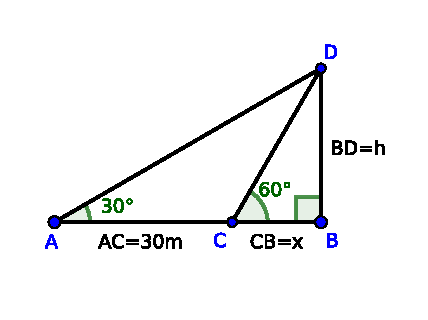
\includegraphics[width=6cm]{Capitulos/Figuras/tri_ret_exer.pdf}

 \end{multicols}
 \end{exer}

 \begin{exer}
 (Sociesc - 2010) Uma rampa lisa de 24 m de comprimento faz ângulo de $60\degree$ com o plano horizontal. Uma pessoa que sobe essa rampa inteira atinge o ponto mais alto verticalmente de:

  Dados: $\sen (60\degree)= \frac{\sqrt{3}}{2}$, $\cos (60\degree)= \frac{1}{2}$, $\tan (60\degree)= \sqrt{3}$
 \begin{multicols}{2}

 \begin{enumerate}
  \item $\frac{17 \sqrt{3}}{2} m$
  \item $15\sqrt{3} m$
  \item $12\sqrt{3} m$
  \item $\frac{25 \sqrt{3}}{2} m$
  \item $18\sqrt{3} m$
 \end{enumerate}

 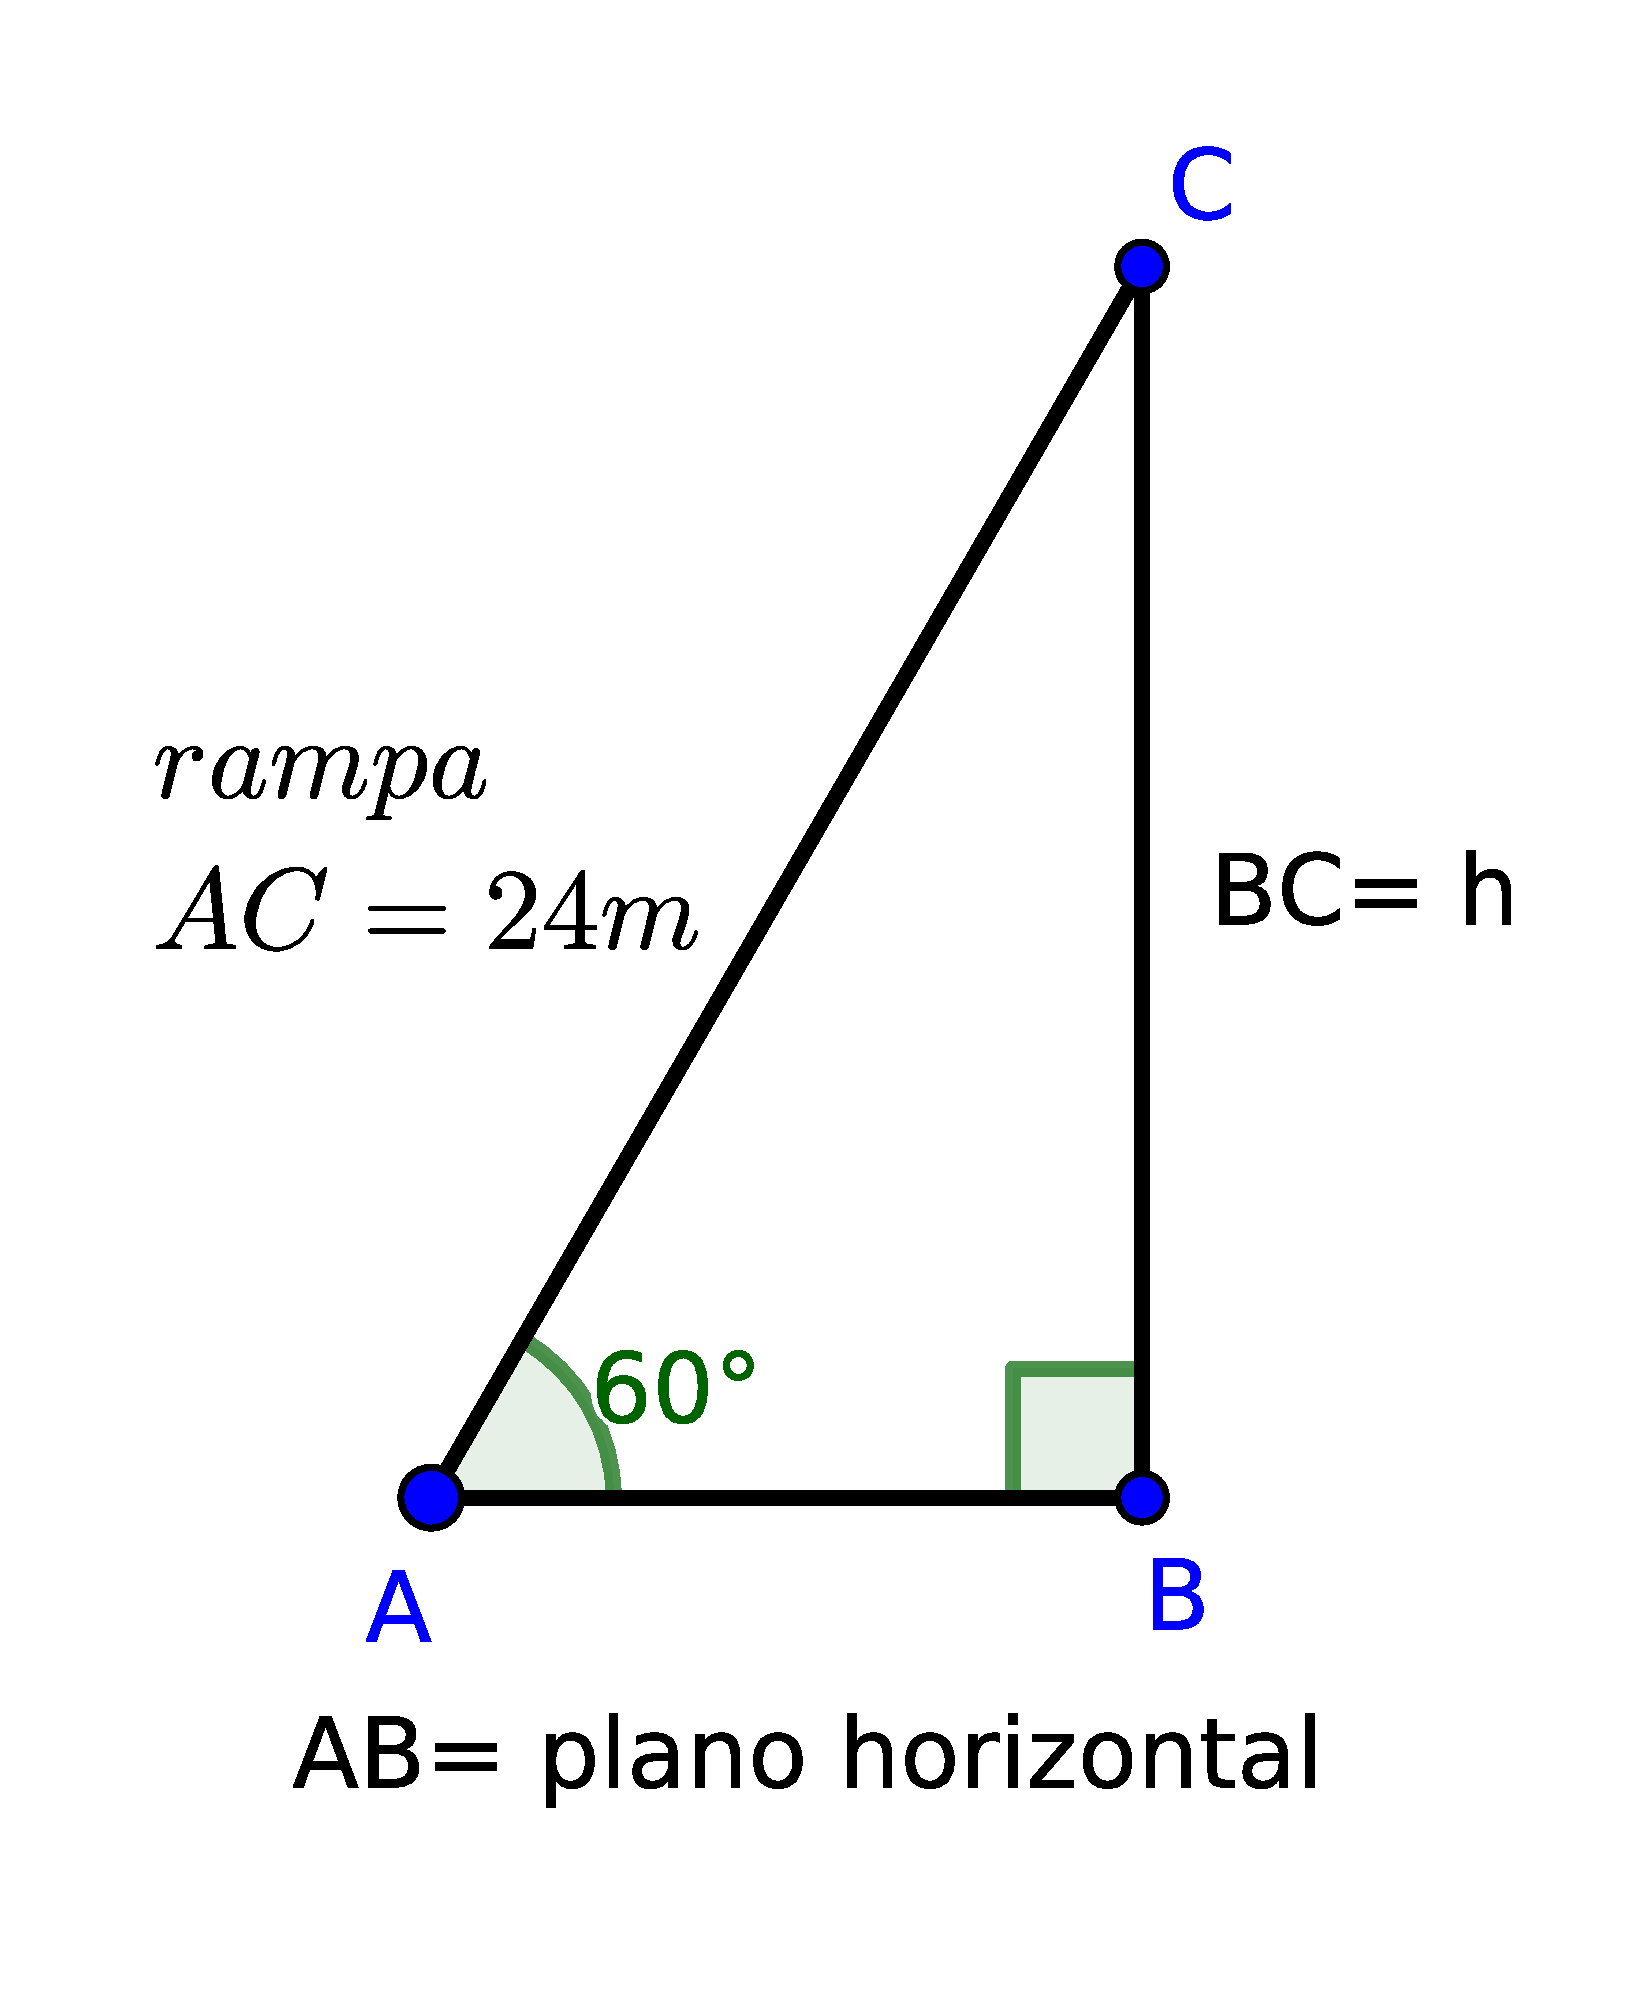
\includegraphics[width=4cm]{Capitulos/Figuras/tri_ret_exer2.pdf}
 \end{multicols}
 \end{exer}

 \begin{exer}
 (Sociesc - 2010) Um teleférico deve unir os topos A e B de dois morros. Para calcular a quantidade de cabo necessário foi preciso medir a altura dos morros em relação a um plano horizontal, obtendo-se 108m e 144m respectivamente. A seguir, mediu-se o ângulo que a reta $\overline{AB}$ forma com a horizontal, obtendo-se $32\degree$. Calcule a distância entre os pontos A e B, sabendo que $\sen (32\degree)= 0,52$, $\cos (32\degree)= 0,84$ e $\tan (32\degree)= 0,62$.

 \begin{multicols}{2}

 \begin{enumerate}
  \item 18,72 m
  \item 48,23 m
  \item 69,23 m
  \item 78,45 m
 \end{enumerate}

 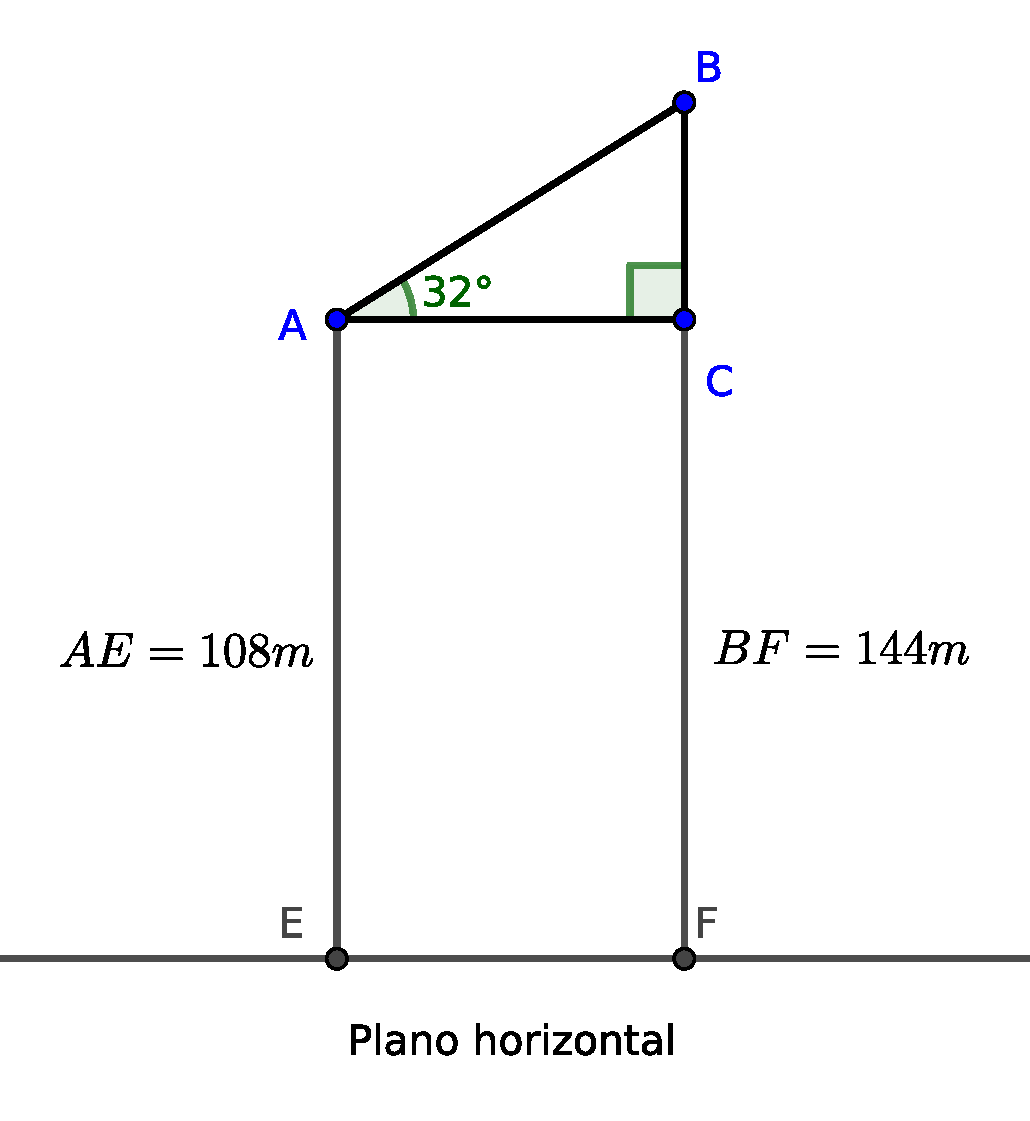
\includegraphics[width=5cm]{Capitulos/Figuras/tri_ret_exer3.pdf}

 \end{multicols}
 \end{exer}

 \begin{exer}
 (Sociesc - 2010) No retângulo abaixo retirou-se dos cantos quatro triângulos retângulos sombreados, formando assim um hexágono regular de lado 4cm.
  \begin{figure}[H]
   \centering
   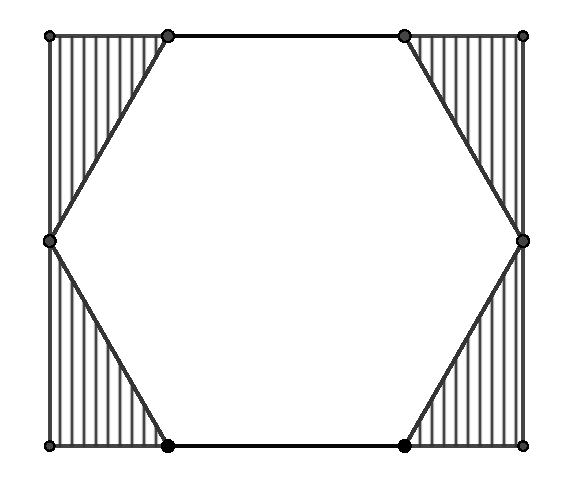
\includegraphics[width=5cm]{Capitulos/Figuras/Hexagono.pdf}
  \end{figure}

  A área do retângulo é:
  \begin{enumerate}
  \item $64cm^2$
  \item $12\sqrt{3}cm^2$
  \item $48cm^2$
  \item $32\sqrt{3}cm^2$
 \end{enumerate}
 \end{exer}

Gabarito: 1 d); 2 c); 3 c); 4 d).

 {\color{red} Nota:} cada ângulo interno de um hexágono mede $120\degree$.
 Pois,
 \vskip0.3cm
\colorbox{azul}{
 \begin{minipage}{0.9\linewidth}
 \begin{center}
 A soma dos ângulos internos de um polígono regular de $n$ lados é dada por:
  \[S= (n-2)\cdot 180 \degree .\]
 \end{center}
 \end{minipage}}
 \vskip0.3cm
 assim, como o hexágono é um polígono regular de $n= 6$ lados, decorre que a soma de seus ângulos internos é:
 \[S= (6-2)\cdot 180= 4 \cdot 180= 720 \degree\]
 portanto, cada ângulo interno $\alpha$ do hexágono mede:
 \[\alpha= \frac{720}{6}= 120 \degree .\]

  \chapter{Funções trigonométricas}

  As funções trigonométricas fazem parte do grupo de funções periódicas, que são as funções que satisfazem a seguinte definição.

  \begin{defi}
   Uma função $f: \R \rightarrow \R$ é denominada \textbf{periódica} quando existe um número real positivo $P$ tal que
   \[f(x + P)= f(x)\]
   para todo $x$ no domínio da $f$. O menor número real positivo $P$ que satisfaz esta propriedade é denominado período de $f$.
  \end{defi}

  Vamos definir as funções trigonométricas no maior subconjunto real possível, e estudar o comportamento de seus gráficos.

  \todo{ períodos, amplitude, intervalo de bijetividade, função inversa}

  \begin{itemize}
  \item Função Seno: $f: \R \rightarrow [-1, 1]$ dada por $f(x)= \sen (x)$, cujo gráfico é:

  \begin{figure}[H]
  \centering
    \fbox{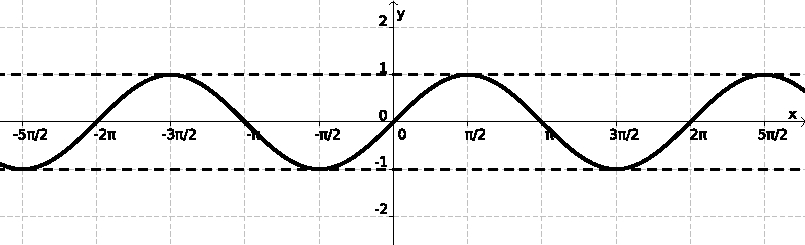
\includegraphics[width=10cm]{Capitulos/Figuras/sen.pdf}}
    \caption{Gráfico da função $f(x)= \sen(x)$}
  \end{figure}

  \item Função Cosseno: $f: \R \rightarrow [-1, 1]$ dada por $f(x)= \cos(x)$, cujo gráfico é:

  \begin{figure}[H]
  \centering
    \fbox{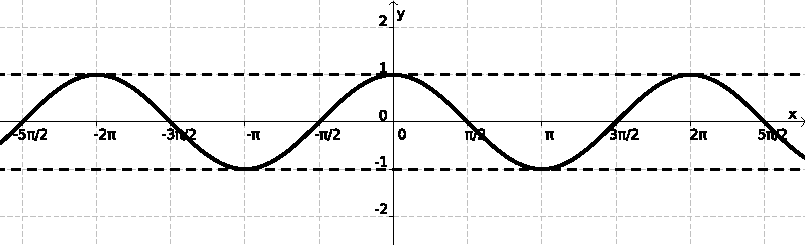
\includegraphics[width=10cm]{Capitulos/Figuras/cos.pdf}}
    \caption{Gráfico da função $f(x)= \cos(x)$}
  \end{figure}

  Geometricamente podemos observar que o comportamento do gráfico das funções seno o cosseno no intervalo $[0, 2\pi]$ se repete em cada intervalo de comprimento $2\pi$. Isso pode ser visualizado também olhando para o círculo trigonométrico, por exemplo quando estamos olhando para um ângulo $\theta= 4\pi + \frac{\pi}{4}$ estamos apenas dando duas voltas no círculo trigonométrico e andando mais $\frac{\pi}{4}$, por isso:
  \[\sen(4\pi + \frac{\pi}{4})= \sen(\frac{\pi}{4}) \ ,\]
  \[\cos(4\pi + \frac{\pi}{4})= \cos(\frac{\pi}{4}) \ , \]
  funções com esta propriedade de repetição de comportamento são denominadas funções periódicas, e o intervalo que se repete é chamado de período.

  Por interpretação do círculo trigonométrico vemos que, para todo $x \in \R$:
  \[\sen(x + 2 \pi)= \sen(x) \ ,\]
  \[\cos(x + 2\pi)= \cos(x) \ , \]
  logo as funções seno e cosseno são de fato funções períodicas de período $2\pi$.

  \item Função Tangente: $f: \R \setminus \{\frac{k\pi}{2} | k \in \Z\} \rightarrow \R$ dada por $f(x)= \tan(x)$, cujo gráfico é:

  \begin{figure}[H]
  \centering
    \fbox{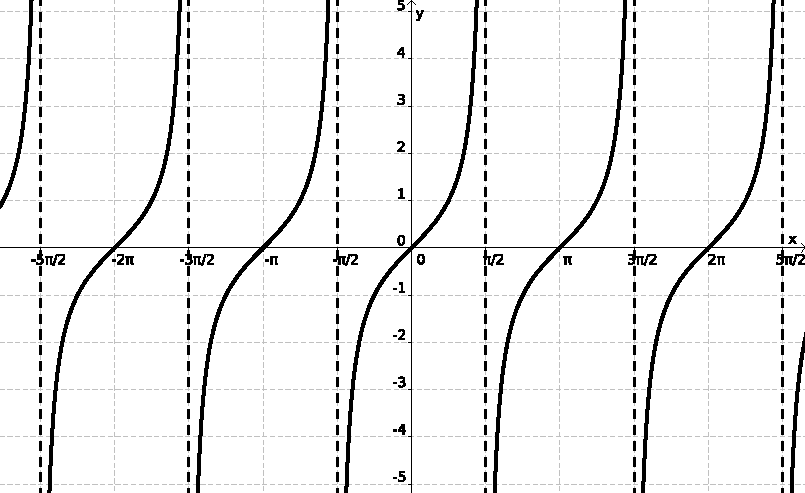
\includegraphics[width=10cm]{Capitulos/Figuras/tan.pdf}}
    \caption{Gráfico da função $f(x)= \tan (x)$}
  \end{figure}

  Lembramos que $\tan(x)= \frac{\sen(x)}{\cos(x)}$, logo podemos entender o domínio da função tangente como o conjunto dos $x \in \R$ tais que $\cos(x) \neq 0$.

  Note que o comportamento do gráfico da função tangente no intervalo $]-\frac{\pi}{2}, \frac{\pi}{2}[$ se repete indefinadamente, e ainda
  \[\tan(x)= \tan(x + \pi)\]
  donde concluímos que a função tangente é uma função períodica de período $\pi$.

  \item Função Cossecante: $f: \R \setminus \{ k\pi | k \in \Z\} \rightarrow \R$ dada por $f(x)= \csc(x)$, o gráfico desta função é:

  \begin{figure}[H]
  \centering
    \fbox{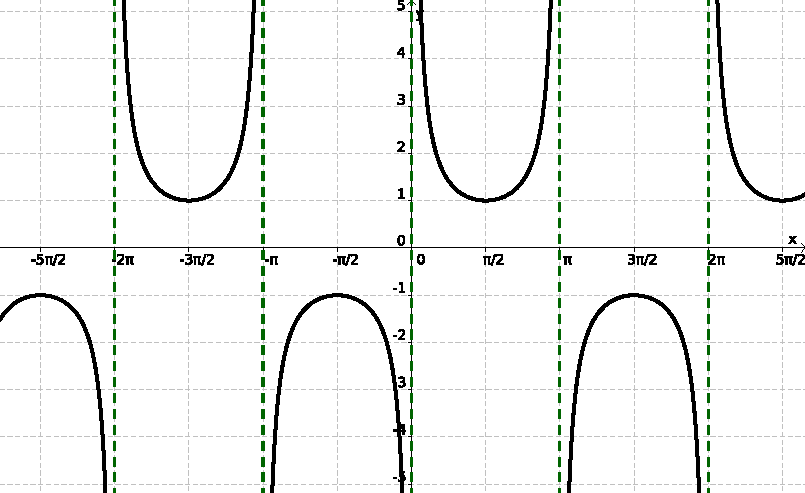
\includegraphics[width=10cm]{Capitulos/Figuras/csc.pdf}}
    \caption{Gráfico da função $f(x)= \csc(x)$}
  \end{figure}

  Como $\csc(x)= \dfrac{1}{\sen(x)}$ o domínio da função cossecante é exatamente o conjunto dos $x \in \R$ tais que $\sen(x) \neq 0$.

  Ao observar o gráfico da função cossecante notamos que o gráfico da função no intervalo $]0, \pi[ \cup ] \pi, 2 \pi[$ se repete indefinidamente, e ainda
  \[\csc(x + 2\pi)= \csc(x) \ , \]
  logo esta é uma função periódica, com período $2\pi$.

  \item Função Secante: $f: \R \setminus \{\frac{k\pi}{2} | k \in \Z\} \rightarrow \R$ dada por $f(x)= \sec(x)$, com gráfico dado por:

  \begin{figure}[H]
  \centering
    \fbox{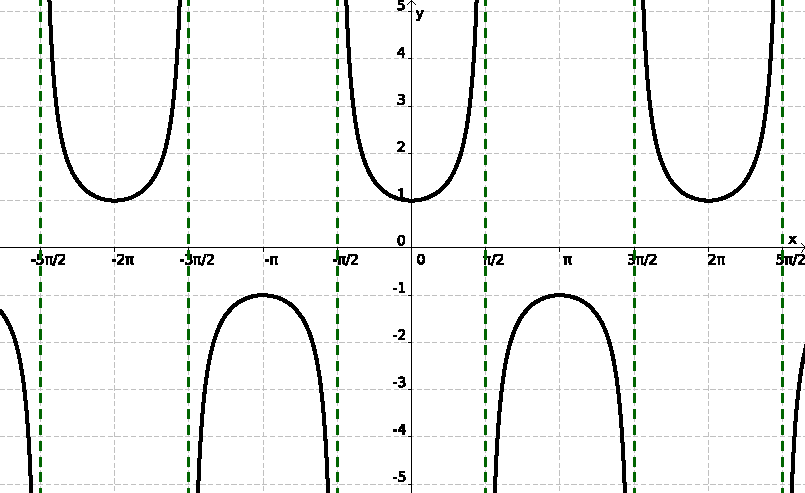
\includegraphics[width=10cm]{Capitulos/Figuras/sec.pdf}}
    \caption{Gráfico da função $f(x)= \sec(x)$}
  \end{figure}

  Como $\sec(x)= \dfrac{1}{\cos (x)}$ o domínio da função secante é o conjunto dos $x \in \R$ tais que $\cos(x) \neq 0$.

  Ao observar o gráfico da função secante notamos que o intervalo que se repete neste caso é $]\frac{-\pi}{2}, \frac{\pi}{2}[ \cup ] \frac{\pi}{2}, \frac{3\pi}{2}[$, e ainda que
  \[\sec(x + 2\pi)= \sec(x) \ ,\]
  logo esta é uma função periódica com período $2\pi$.

  \item Função Cotangente: $f: \R \setminus \{ k\pi | k \in \Z\} \rightarrow \R$ dada por $f(x)= \cotan(x)$, cujo gráfico é:

  \begin{figure}[H]
  \centering
    \fbox{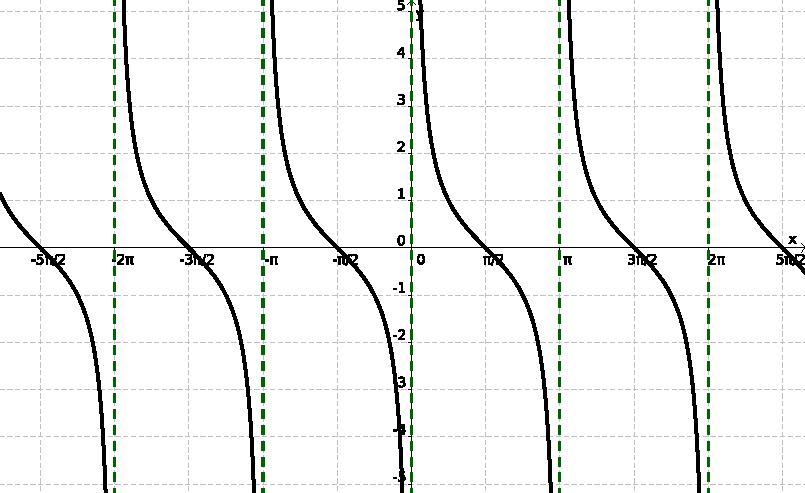
\includegraphics[width=10cm]{Capitulos/Figuras/cot.pdf}}
    \caption{Gráfico da função $f(x)= \cotan(x)$}
  \end{figure}

  Lembramos que $\cotan(x)= \dfrac{\cos(x)}{\sen(x)}$ logo o domínio da função cotangente é o conjunto dos $x \in \R$ tais que $\sen(x) \neq 0$.

  Já no gráfico da função cotangente vemos a repetição do comportamento do intervalo $]0, \pi[$, e temos que
  \[\cotan(x + \pi)= \cotan(x)\]
  portanto esta é uma função periódica de período $\pi$.

  \textbf{Funções Inversas}

  As funções trigonométricas admitem inversas quando restringimos seus domínios a um único período da função, assim temos por exemplo as seguintes funções:

  \item Função Arco Seno: $f: [-1, 1] \rightarrow [\frac{-\pi}{2}, \frac{\pi}{2}]$ dada por $f(x)= \arcsen(x)$, que também denotamos por $\sen^{-1}(x)= \arcsen(x)$, neste caso o gráfico será:

  \begin{figure}[H]
  \centering
    \fbox{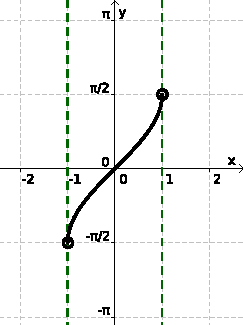
\includegraphics[width=5cm]{Capitulos/Figuras/arcsen.pdf}}
    \caption{Gráfico da função $f(x)= \arcsen(x)$}
  \end{figure}


  \item Função Arco Cosseno: $f: [-1, 1] \rightarrow [0, \pi]$ dada por $f(x)= \arccos(x)$, que também denotamos por $\cos^{-1}(x)= \arccos (x)$, neste caso temos o seguinte gráfico:

  \begin{figure}[H]
  \centering
    \fbox{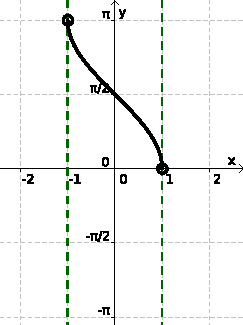
\includegraphics[width=5cm]{Capitulos/Figuras/arccos.pdf}}
    \caption{Gráfico da função $f(x)= \arccos(x)$}
  \end{figure}


  \item Função Arco Tangente: $f: \R \rightarrow ]\frac{-\pi}{2}, \frac{\pi}{2}[$, dada por $f(x)= \arctan(x)$ que também denotamos por $\tan^{-1}(x)= \arctan (x)$, neste caso o gráfico será:

  \begin{figure}[H]
  \centering
    \fbox{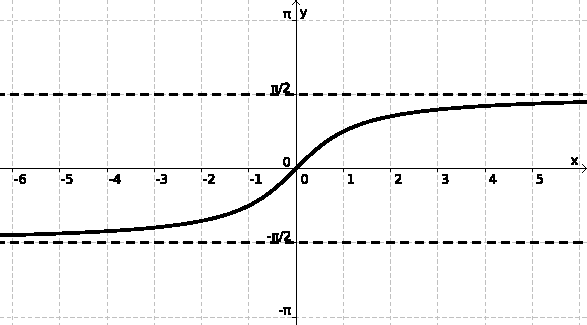
\includegraphics[width=10cm]{Capitulos/Figuras/arctan.pdf}}
    \caption{Gráfico da função $f(x)= \arctan(x)$}
  \end{figure}


  \end{itemize}
